\documentclass[12pt]{article}

%\usepackage{fancyhdr}	% header y footer

% Márgenes 
\topmargin=-0.45in      %
\evensidemargin=0in     %
\oddsidemargin=0in      %
\textwidth=6.5in        %
\textheight=9.0in       %
\headsep=0.25in         %

% Acentos en castellano
% \usepackage[latin1]{inputenc} % iso-8889-1
\usepackage[utf8]{inputenc} % utf-8

\usepackage{graphicx}	% imagenes
% Soporte para hyperlinks.

\usepackage{hyperref}

\usepackage[T1]{fontenc}
\usepackage{mathtools}

% Temporal para las anotaciones de cosas a rellenar
\usepackage{color}
\usepackage{listings}             % Para poner código
\usepackage{natbib}

\usepackage{color}
\usepackage{subcaption}


\definecolor{mygreen}{rgb}{0,0.6,0}
\definecolor{mygray}{rgb}{0.5,0.5,0.5}
\definecolor{mymauve}{rgb}{0.58,0,0.82}
\definecolor{light-gray}{gray}{0.95}

\lstset{ %
  backgroundcolor=\color{light-gray},   % choose the background color; you must add \usepackage{color} or \usepackage{xcolor}
  basicstyle=\footnotesize,        % the size of the fonts that are used for the code
  breakatwhitespace=false,         % sets if automatic breaks should only happen at whitespace
  breaklines=true,                 % sets automatic line breaking
  captionpos=b,                    % sets the caption-position to bottom
  commentstyle=\color{mygreen},    % comment style
  deletekeywords={...},            % if you want to delete keywords from the given language
  escapeinside={\%*}{*)},          % if you want to add LaTeX within your code
  extendedchars=true,              % lets you use non-ASCII characters; for 8-bits encodings only, does not work with UTF-8
  %frame=single,                    % adds a frame around the code
  keepspaces=true,                 % keeps spaces in text, useful for keeping indentation of code (possibly needs columns=flexible)
  keywordstyle=\color{blue},       % keyword style
  language=C,                 % the language of the code
  morekeywords={*, ..., For, If, :=>, <=, free, function, While},            % if you want to add more keywords to the set
  numbers=left,                    % where to put the line-numbers; possible values are (none, left, right)
  numbersep=5pt,                   % how far the line-numbers are from the code
  numberstyle=\tiny\color{mygray}, % the style that is used for the line-numbers
  rulecolor=\color{black},         % if not set, the frame-color may be changed on line-breaks within not-black text (e.g. comments (green here))
  showspaces=false,                % show spaces everywhere adding particular underscores; it overrides 'showstringspaces'
  showstringspaces=false,          % underline spaces within strings only
  showtabs=false,                  % show tabs within strings adding particular underscores
  stepnumber=1,                    % the step between two line-numbers. If it's 1, each line will be numbered
  stringstyle=\color{mymauve},     % string literal style
  tabsize=2,                       % sets default tabsize to 2 spaces
  title=\lstname                   % show the filename of files included with \lstinputlisting; also try caption instead of title
}




% Nombres de contenido generado automáticamente (como tabla de contenidos)
% en español. Para poder usarlo:
% sudo apt-get install texlive-lang-spanish
%
% Comentado mientras no sea necesario para nada mas; podemos cambiar
% el nombre de la tabla de contenidos a mano, puesto que este paquete
% parece que fuerza los números de página románicos a ser en mayúscula.
\usepackage[spanish]{babel}

\begin{document}

\title{
	{\bf Neurocomputación} \\
	Práctica 1:\\ {\bf Redes de McCulloh-Pitch. Perceptrón y Adaline}.\\
}
\author{
	Daniel Gutiérrez Navío \\
	Matías Bender \\
	\textit{Grupo 2461}
}
\date{\today}

\maketitle

% necesario quitar el estilo de página después de \maketitle para quitar el
% primer numero de pagina, porque \maketitle hace \pagestyle{plain}
\thispagestyle{empty}
\newpage

% numeración romana para las primeras páginas
\pagenumbering{roman}

%\renewcommand*\contentsname{Índice}
\tableofcontents
\listoffigures
\newpage

\bibliographystyle{alpha}
%\bibliography{sample}

% numeración arábica para el resto del documento
\setcounter{page}{1}
\pagenumbering{arabic}

% indentacion primera linea de parrafo
\setlength{\parindent}{0pt}

% distancia entre parrafos
\setlength{\parskip}{8pt}

% Parte 1: Manual de uso (si se necesita)
%%%%%%%%%%%%%%%%%%%%%%%%%%%%%%%%%%%%%%%%%%%%%%%%%%%%%%%%%%%%%%%%%%%%%%%%%%%
%el section del manual se pone como está comentado aquí, para que salga sin número pero en el índice
%\phantomsection
%\addcontentsline{toc}{section}{Manual de uso}
%\section*{Manual de uso}

\newpage
% Introducción
%%%%%%%%%%%%%%%%%%%%%%%%%%%%%%%%%%%%%%%%%%%%%%%%%%%%%%%%%%%%%%%%%%%%%%%%%%%
\section*{Introducción}
\addcontentsline{toc}{section}{Introducción}
Esta práctica, la primera de la asignatura de Neurocomputación, se tratará de conseguir una aproximación a redes neuronales, mediante la codificación de tres de las primeras redes neuronales: perceptrón simple, adaline, y red de McCulloh-Pitts, para la resolución de los problemas propuestos.

\subsection*{Diseño}
Para la resolución de esta práctica, y de las venideras, hemos decidido realizar el desarrollo de una interfaz para redes neuronales en C++, para simplificar futuros trabajos. 
La interfaz principal, está compuesta de estructuras de neuronas y links. Una neurona es una simple unidad, con entrada y salida de datos, y un proceso adaptable para la transformación de una en otra.

El link, es un enlace pesado entre dos neuronas, que lleva la salida, multiplicada por su peso, a la entrada del objetivo, donde suma a lo que ya haya.

Mediante estos dos elementos, podemos construir cualquier red neuronal.
Además, se ha diseñado una clase, perceptrón, con una estructura genérica adaptable, que puede usarse para la construcción de otras redes.

\newpage
% 1 McCulloh-Pitch
%%%%%%%%%%%%%%%%%%%%%%%%%%%%%%%%%%%%%%%%%%%%%%%%%%%%%%%%%%%%%%%%%%%%%%%%%%%
\section{Transformada rápida de Fourier con recursión}
%Descripción del algoritmo FFT con recursión. 
En este apartado de la práctica, se deberá realizar una red de McCulloh-Pitts para la resolución del problema propuesto.
Se utilizará la siguiente arquitectura de McCulloh-Pitts para realizar la red:

\begin{figure}[h!]
    \label{fig:fig1}
  \centering
       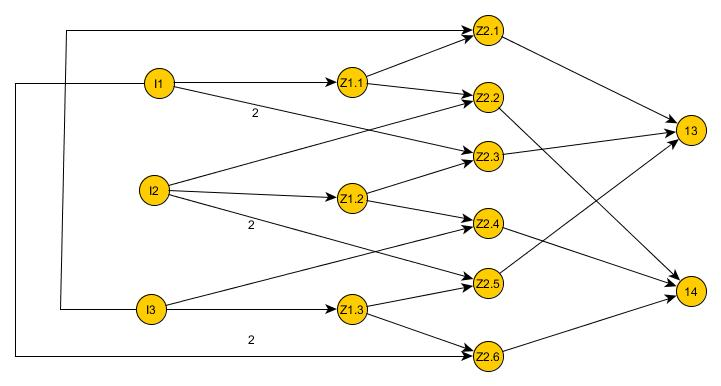
\includegraphics[width=0.7\textwidth]{recursos/fig1}
    \caption{Red de McCulloh-Pitch}
\end{figure} 

Usando como umbral en todas las neuronas 2, y sin usar ninguna sinapsis inhibitoria.

La implementación de esta red, como puede verse, se ha hecho de manera totalmente lineal, creando una estructura en capas, en las que no existe ningún tipo de retroalimentación, sino que una capa inferior proporciona salidas conectadas a las capas superiores (no a la inmediatamente superior necesariamente).

En nuestro caso, usamos 4 capas: una capa de entrada, una capa de salida, y 2 niveles de capas ocultas, provocando así un retraso de 3 épocas entre una entrada, y su correspondiente salida.

En caso de no haber entrada dado que no se ha cargado aún, el sistema devolverá 0 0 0, la salida neutra, que no proporciona ningún tipo de información.

Se han diseñado distintos ejemplos, y sus salidas, que pueden verse en el makefile escribiendo \texttt{makefile help-mcculloh}.

\newpage

% 2 Perceptrón y Adaline
%%%%%%%%%%%%%%%%%%%%%%%%%%%%%%%%%%%%%%%%%%%%%%%%%%%%%%%%%%%%%%%%%%%%%%%%%%%
\section{Perceptrón y Adaline}
\subsection*{Introducción}
En esta parte, se deberá realizar la implementación de dos algoritmos nuevos: un Perceptrón de capa simple, y un Adaline. Ambos redes neuronales simples para problemas lineales.

En ambos casos, son algoritmos de aprendizaje supervisado, que requieren de un tiempo de preparación, llamado entrenamiento, para su correcto funcionamiento.

\subsection{Perceptrón}

\subsubsection{Introducción y diseño}

El objetivo de este ejercicio consiste en construir un perceptrón simple, o monocapa, con una sola neurona de salida, para reconocer patrones. Usaremos la estructura de red neuronal que hemos descrito al principio de este documento, pero adaptandola al sistema de entrenamiento y clasificación de un perceptrón.

Este sistema consiste en aplicar una variación de la regla de hebb, es decir, en caso de error en clasificar un elemento de entrenamiento, aplicaremos una actualización de pesos. La actualización de pesos que aplicaremos será la siguiente:
$w_{t+1}=w_{t}+ \alpha*t*x$

Donde w, es el peso de la sinapsis en un momento concreto, $\alpha$ es la constante de entrenamiento $(0 < \alpha \ge 1)$, y t es un valor de verdad, que corresponde a la clase que es de verdad (1 si es clase 1, -1 si es clase 2, al ser bipolar).

Decidimos usar de condición de parada, un 100\% de acierto, es decir, una etapa completa sin un solo error. Pero como muy a menudo, al poder clasificar solo problemas lineares, esto no es posible, hemos decidido una cantidad de épocas de entrenamiento. Usaremos una cantidad de épocas elevada, 100, aunque luego comentaremos esta cantidad y miraremos los problemas acotados en caso de que se detenga el proceso de aprendizaje.

\subsubsection{Descripción de los resultados}
Tras preparar el perceptrón de la manera que se ha explicado, ejecutamos el programa para obtener datos estadísticos de el proceso de aprendizaje.

El resultado, es de un 93\% de acierto en entrenamiento, que cambia a 95\% de acierto en el testing.

El resultado, como podemos comprobar, es realmente muy eficaz, dado que podemos ver que se adapta de una manera muy buena a el problema propuesto.

En la siguiente gráfica, podemos apreciar la evolución durante el entrenamiento (acotado).

\begin{figure}[h!]
    \label{fig:fig2}
  \centering
       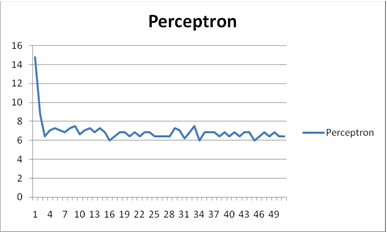
\includegraphics[width=0.7\textwidth]{recursos/fig2}
    \caption{Evolución del entrenamiento del perceptrón}
\end{figure} 

Podemos comprobar, que se mantiene constante gran parte del tiempo el error, por lo que podemos determinar que, usando un perceptrón, no podemos superar cierta cota en este problema de error, suponiendolo a ruido o casos no lineales.


\subsection{Adaline}

\subsubsection{Introducción y diseño}

En este ejercicio, se nos pide modificar la red creada en el anterior, el perceptrón, para crear un Adaline. El adaline es una red neuronal, basada también en aprendizaje de Hebb, pero con graves modificaciones, para orientarse a la reducción del error cuadrático medio.
El error cuadrático medio (ecm), es una medida usada para el error promedio en estimación. Para calcularlo, se tiene que encontrar el valor esperado del cuadrado de la diferencia entre <X> (el estimador), y X, aplicando la fórmula:

$ecm = \frac{sqrt(sum(xi-<X>)^{2})}{n}$

siendo <X>, $(\frac{sum(x_{i})}{n})$, podemos sustituir, dándonos la fórmula

$ecm = \frac{sqrt(sum(xi-(\frac{sum(x_{i})}{n}))^{2}}{n}$

La regla que reduce este error, se obtiene mediante su gradiente, dándo a usar la conocida como llamada regla delta para la actualización de pesos:

$w_{i+1} = w_{i} + \alpha*(t-y)*x$

Esta regla, a diferencia del perceptrón, que solo actualiza en caso de error, se aplica siempre.

\subsubsection{Descripción de los resultados}

Para exponer los resultados, usaremos la misma estructura que empleamos en el caso del perceptrón, solo que además añadiremos una gráfica exponiendo la variación del error cuadrático medio, para observar la eficacia de este algoritmo (cosa que no se hizo en el perceptrón, al no ser considerado relevante para el problema, ya que el perceptrón ignora (aunque afecta indirectamente) el error cuadrático medio, y no es motivo de comparación).

El resultado del entrenamiento, con un máximo de épocas acotado, es el siguiente, viéndolo comparativamente el ECM con el error:

\begin{figure}[h!]
    \label{fig:fig1}
  \centering
       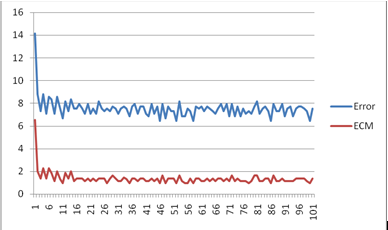
\includegraphics[width=0.7\textwidth]{recursos/fig8}
    \caption{Adaline: ECM vs Error}
\end{figure} 

El error al final del entrenamiento, como ha podido apreciarse, es de XXX\%, mientras que en el test, es de XXX\%. Esto, como se mencionó, varía con cada ejecución al hacerse una distribución aelatoria de los datos.

\subsection{Parámetros de aprendizaje}

Para realizar este ejercicio, mostraremos una tabla con los resultados de variar, con un máximo de 100 épocas, la constante de aprendizaje entre 0,1 y 1, tanto en adaline como en pereceptrón.

\begin{figure}[h!]
    \label{fig:fig1}
  \centering
       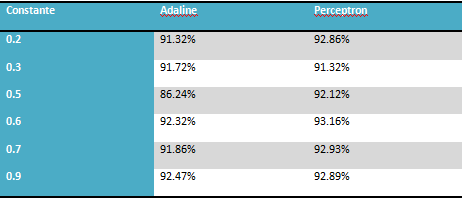
\includegraphics[width=0.7\textwidth]{recursos/fig9}
    \caption{Constantes de aprendizaje}
\end{figure} 

Como se puede ver, al no llegar a converger nunca, no se ha podido comprobar exactamente el efecto. Sin embargo, se ha podido apreciar que tarda más en estabilizarse cuanto menor es la constante de aprendizaje (la diferencia sin embargo, no es demasiado considerable en este intervalo).

\subsection{Entrenamiento-test completo}
La variación se ha realizado, haciendo que pueda recibir el main 2 argumentos, un primer argumento que sea el conjunto de entrenamiento, y otro segundo argumento, el de test. En caso de ser de conjuntos distintos, el programa no se hace responsable y DARÁ MUY PROBABLEMENTE UN ERROR.

A continuación se muestra el resultado de analizar los archivos propuestos, con número de épocas hasta la convergencia, en caso de existir (límite: 100 epocas).

\newpage
\subsubsection*{NAND}
\begin{figure}[h!]
    \label{fig:fig3}
  \centering
       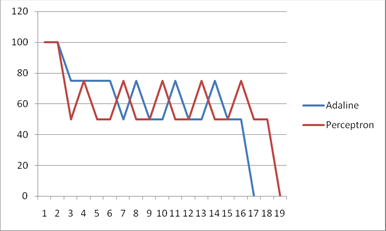
\includegraphics[width=0.7\textwidth]{recursos/fig3}
    \caption{NAND}
\end{figure} 



\subsubsection*{NOR}
\begin{figure}[h!]
    \label{fig:fig4}
  \centering
       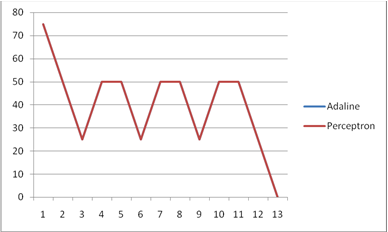
\includegraphics[width=0.7\textwidth]{recursos/fig4}
    \caption{NOR}
\end{figure} 

Nótese que aquí ambas coinciden
\subsubsection*{XOR}
\begin{figure}[h!]
    \label{fig:fig5}
  \centering
       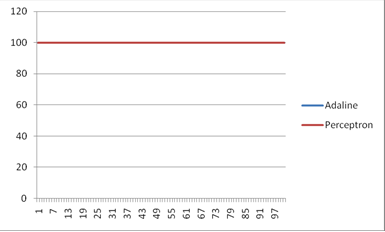
\includegraphics[width=0.7\textwidth]{recursos/fig5}
    \caption{XOR}
\end{figure} 

Podemos observar que aquí siempre da error. Podría dar al principio algún caso de éxito, dependiendo de los valores iniciales.

Como podemos comprobar, xor no llega a ninguna convergencia. Esto es debido a que xor no es linealmente separable, mientras que los demás al ser linealmente separables, si que pueden ser resueltos completamente.

\subsection{Clasificación de datos desconocidos}
Se ha aplicado el problema propuesto tanto al perceptrón como al adaline. Se muestran a continuación las gráficas de entrenamiento (acotadas a 100 epocas), de ambos, en el caso de usar con una división 2/3 training, 1/3 test, en el archivo problema\_real2.txt.

La gráfica de la evolución de el entrenamiento en perceptrón y adaline es la siguiente:
\begin{figure}[h!]
    \label{fig:fig6}
  \centering
       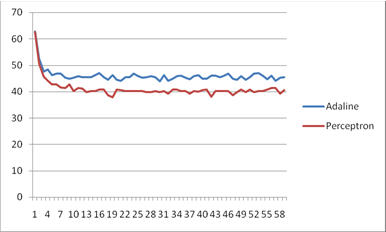
\includegraphics[width=0.7\textwidth]{recursos/fig6}
    \caption{Evolución del entrenamiento del Perceptrón y Adaline}
\end{figure} 

En ella podemos ver que el perceptrón tiene un índice de error menor que el adaline. Eso es debido a que el perceptrón funciona pensando en el error final, mientras que el adaline en el error cuadrático medio, siéndo este visiblemente más suave.

Por último, se muestra a continuación las gráficas de entrenamiento de usar el fichero entero como entrenamiento. Los resultados de el problema, irán en un archivo adjunto a esta memoria.
\begin{figure}[h!]
    \label{fig:fig7}
  \centering
       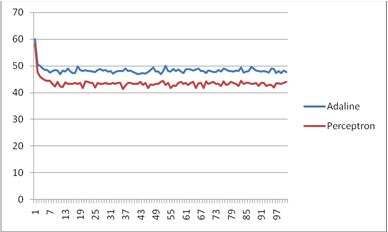
\includegraphics[width=0.7\textwidth]{recursos/fig7}
    \caption{Evolución del entrenamiento 'completo' del Perceptrón y Adaline}
\end{figure} 

En ella se puede ver un desarrollo similar a la anterior, en la que el perceptrón muestra, durante el entrenamiento, un mejor comportamiento que el adaline, al tener casi un 10\% de acierto más que el adaline.


\subsection{Añadir parámetros no lineales}
Este ejercicio no es propiamente un ejercicio, ya que basta con añadir unos cuantos datos aleatorios, que sean no lineales (ruido). Para ello, hemos introducido en los datos ciertos datos que nos hemos inventado, y hemos observado que la precision empeora, pero al no converger ya de por sí, el impacto es menor del que esperamos.

\newpage
% Conclusiones
%%%%%%%%%%%%%%%%%%%%%%%%%%%%%%%%%%%%%%%%%%%%%%%%%%%%%%%%%%%%%%%%%%%%%%%%%%%
\section*{Conclusiones}
\addcontentsline{toc}{section}{Conclusiones}

En esta práctica hemos aprendido a implementar redes neuronales para la resolución de sistemas lineales ( o problemas lineales ). Pese a la utilidad de ésto, teóricamente, en la realidad, como se ha podido comprobar durante la práctica, los problemas lineales no son demasiado comunes, por lo que un sistema imperfecto como éste no tiene demasiada utilidad en un caso real (ruido, así como complejidad de los problemas). Sin embargo, estos algoritmos luego servirán de base para otros más potentes con capacidad de división no lineal.

Además, en esta práctica hemos creado, en el lenguaje de programación \verb!C++!, un "framework" de redes neuronales, para realizar una arquitectura de redes neuronales genéricas, que nos servirá en las siguientes prácticas.


% (OPTATIVO) 4 Aplicación de la transformada discreta de Fourier sobre una señal.
%%%%%%%%%%%%%%%%%%%%%%%%%%%%%%%%%%%%%%%%%%%%%%%%%%%%%%%%%%%%%%%%%%%%%%%%%%%
%\section{Ejercicio 4: Aplicación de la transformada discreta de Fourier sobre una señal.}
%Breve descripción de la TDF indicando tres aplicaciones prácticas. Asimismo, se deberá explicar el significado de la serie transformada respondiendo a las siguientes preguntas:
%-	¿En qué puntos de la serie transformada aparecen impulsos y qué módulo tienen? ¿Cómo se relacionan con la señal original?
%-	¿Qué se consigue utilizando filtros de baso bajo y de paso de banda? ¿Qué sucede a la señal original cuando aplicamos filtros de baso bajo y de paso de banda? ¿y cuando eliminamos la componente cero de la serie transformada?
%-	Gráficas de la señal original y de las señales obtenidas tras aplicar los filtros.

%\newpage

% Conclusiones
%%%%%%%%%%%%%%%%%%%%%%%%%%%%%%%%%%%%%%%%%%%%%%%%%%%%%%%%%%%%%%%%%%%%%%%%%%%
%\section*{Conclusiones}





%\addcontentsline{toc}{section}{Conclusiones}


%\newpage



% Para cada prueba se pide una descripción de la misma que incluya: 
	% - nombre de la función a probar
	% - objetivo de la prueba
	% - desarrollo 
	% - resultado esperado


% Detallar los resultados obtenidos tras el paso de las pruebas a la práctica y las conclusiones extraídas de dichos resultados

% 8 Conclusiones
%%%%%%%%%%%%%%%%%%%%%%%%%%%%%%%%

%%%% Consideraciones finales y anexos %%%%%%
%\phantomsection
%\addcontentsline{toc}{section}{Anexo A. Pseudocódigo de Dijkstra}
%\section*{Anexo A. Pseudocódigo de Dijkstra}

% Referencias
%%%%%%%%%%%%%%%%%%%%%%%%%%%%%%%%%%%%%%%%%%%%%%%%%%%%%%%%%%%%%%%%%%%%%%%%%%%

%\bibliographystyle{plain}
%\renewcommand*\refname{Referencias}		% Titulo en español
%\bibliography{recursos/bibliografia}

%TODO: RFC DE IRC (Descomentar)
%\begin{thebibliography}{2}
%\bibitem{1}
%	Network Working Group,
%	\emph{RFC 1459: Internet Relay Chat, IRC}.
%\bibitem{2}
%	Network Working Group,
%	\emph{RFC 2326: RTSP: Real Time Streaming Protocol Overview}.
%\bibitem{3}
%	Network Working Group,
%	\emph{RFC 3550: RTP: A Transport Protocol for Real-Time Applications}.
%\bibitem{4}
%	Network Working Group,
%	\emph{RFC 1889: RTP: A Transport Protocol for Real-Time Applications}.
%\end{thebibliography}


% Figuras
%%%%%%%%%%%%%%%%%%%%%%%%%%%%%%%%%%%%%%%%%%%%%%%%%%%%%%%%%%%%%%%%%%%%%%%%%%%
%\begin{figure}[h!]
%	\centering
%   		 \includegraphics[width=0.7\textwidth]{recursos/Hilos}
%  	\caption{Hilos de la aplicación}
%  	\label{hilos}
%\end{figure} 


\end{document}
